\documentclass[../report.tex]{subfiles}

\begin{document}

\graphicspath{{img/}{../img/}}

\section{Scrum men... Ikke helt}
\label{sec:Scrum}

Target-projektgruppen har valgt at arbejde med Scrum i deres implementeringsfase, hvilket optager cirka halvdelen af deres tidsplan(se Gantt-chart fig \ref{fig:Gantt} side \pageref{fig:Gantt}). I deres Scrum-forl�b blev det besluttet at k�re l�st p� nogle af Scrums discipliner, fordi der var enighed om, at det ikke gav meget mening, for en projektgruppe der kun m�des et par gange om ugen, at k�re fuld Scrum. En forklaring af target-projektgruppens Scrum aktiviteter kan ses i tabel \ref{tab:Scrum}, og de vigtige aktiviteters placering i sprintet kan ses p� figur \ref{fig:ScrumTimeline}.


\begin{figure}[H]
\centering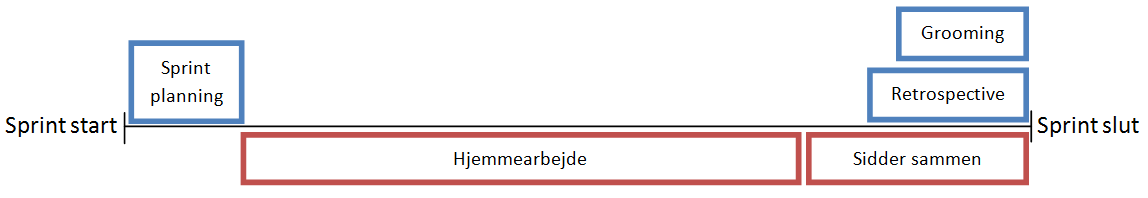
\includegraphics[scale=0.45]{SCRUMtimeLine.png}
\caption{Sprint tidslinje}
\label{fig:ScrumTimeline}
\end{figure}



%\noindent Target-projektgruppens sprints startede s�ledes med sprint planning, efterfulgt af en periode med individuelt arbejde, for s� at afslutte med gruppearbejde hvor Scrumboardet blev groomet og et retrospective p� sprintet udf�rt.


\begin{table}[H]
\begin{tabularx}{15cm}{l|X}
\textbf{Aktivitet}  & \textbf{Beskrivelse} \\
Scrum roller & I et eksamensprojekt er det urealistisk at have en person til kun at v�re product owner. I target-projektet er product owner ene og alene ansvarlig for kommunikation med stakeholders og prioritering af product items, men han er ogs� udvikler i Scrum teamet. Derudover er Scrummaster og developers blevet brugt ligesom i fuld Scrum.     \\ 
 & \\
Sprint & Sprints af 1 uges varighed\\
 & \\
Standup meeting & Der blev ikke afholdt nogen standup meetings. \\
 & \\
Grooming & Den n�stsidste aktivitet var grooming, hvor Scrumboardet blev ryddet op. \\
 & \\
Retrospective & Den sidste aktivitet var retrospective. Gruppen benyttede Keep-Stop-New metoden. \cite{cohn} \\
 & \\
Sprint planning & Den f�rste aktivitet i hvert sprint er en klassisk sprint planning. Tasks blev estimeret med planning poker i points, som beskrevet i afsnit \ref{sec:Delphi} p� side \pageref{sec:Delphi}. \\
 & \\
Scrumboard & Scrum boardet er den centrale oversigt over aktiviteter. Da target-projektgruppen ikke havde et fast lokale allokeret, var et fysisk Scrumboard ikke muligt, s� online v�rkt�jet Trello (se trello.com) blev brugt i stedet. \\
 & \\
Tidtagning & Der blev i fire sprints taget tid p� arbejdet med Toggl (se toggl.com). Det var noget target-projektgruppen blev bedt om, for at der i dette projekt kunne laves analyser af deres tidsforbrug og velocity.
\end{tabularx}
\caption{Target-projektets Scrum aktiviteter}
\label{tab:Scrum}
\end{table}

\newpage

\subsection{Udtalelser fra target-projektgruppen}

\noindent Target-projektgruppen har ikke brugt Scrum i hele deres projektforl�b, men det kunne de godt have valgt at g�re. De udtaler f�lgende:

\begin{quote}
\textit{
	"Grunden til at vi ikke har brugt Scrum fra projektstart er, at vi f�lte en hvis struktur af dokumentationen var n�dvendig. Vi har alts� set p� Scrum som en implementerings procesmodel. I vores Scrum-forl�b har vi dog ogs� haft andet end implementeringstasks, og vi kan sagtens se gevinster ved at bruge Scrum fra projektstart."}
\label{cite:Scrumstart}
\end{quote}

\noindent Et andet interessant punkt er valget af Scrum aktiviteter, og gruppen udtaler f�lgende:

\begin{quote}
\textit{
	"F�rst og fremmest m� det siges at vi har v�ret tilfredse med vores form p� Scrum. Det kan vi sige rimeligt sikkert fordi vi l�bende via vores retrospectives har kunne rette til i processen. Med det har vi for eksempel afpr�vet ikke at estimere tasks i de sidste to sprints, og det har vist os at estimeringen er vigtig fordi; tvinger en dialog om indholdet af en task, og viser mere pr�cist hvor meget arbejde et sprint indeb�rer. \\
	Den vigtigste ting med Scrum har for os v�res sprint l�ngden, som vi har holdt p� en uge. Fordelen ved disse sprints over et vandfaldsforl�b er at man hele tiden holder individer op p� deres arbejde - Det er nemlig ogs� en stor motivationsfaktor at man hver uge skal have nogle ting klar, eller en forklaring for hvorfor man ikke har.
}
\end{quote}

\noindent Med disse udtalelser p� plads vil der g�s videre til n�ste afsnit som omhandler vandfaldsmodellen som alternativ




\end{document}